\documentclass[12pt, a4paper]{article}
\usepackage[UTF8]{ctex}

% 删除CTeX章节定制,改用titlesec包
\usepackage{titlesec}

% 章节样式定义
\titleformat{\section}[hang]
  {\Large\bfseries\color{darkacademic}}
  {\thesection.}{0.5em}{}
\titlespacing*{\section}
  {0pt}{1em}{0.5em}

\titleformat{\subsection}[hang]
  {\large\bfseries\color{academicblue}}
  {\thesubsection}{0.5em}{}
\titlespacing*{\subsection}
  {0pt}{0.8em}{0.3em}

\usepackage{geometry}
\usepackage{fancyhdr}
\usepackage{graphicx}
\usepackage{amsmath}
\usepackage{amsfonts}
\usepackage{amssymb}
\usepackage{array}
\usepackage{setspace}
\usepackage{enumitem}  % 用于自定义目录编号格式
\usepackage{xcolor}
\usepackage{tikz}
\usepackage{tcolorbox}
\tcbuselibrary{most}
\usepackage[colorlinks=true, linkcolor=darkblue, citecolor=darkblue, urlcolor=blue]{hyperref}
\usepackage{bookmark}
\usepackage{listings}
\usepackage{xcolor}    % 代码高亮配色
\lstset{
    backgroundcolor=\color{lightgray},
    basicstyle=\ttfamily\small,
    keywordstyle=\color{academicblue},
    commentstyle=\color{accentgray},
    stringstyle=\color{red},
    showstringspaces=false,
    breaklines=true,
    numbers=left,
    numberstyle=\tiny,
    frame=single,
    language=C++
}

% 改善自动换行和断词
\usepackage{microtype}  % 改善文字排版质量
\usepackage{xurl}       % 允许在任意位置断开URL和代码
\sloppy                 % 允许更宽松的行间距以避免溢出

% 定义学术风格颜色
\definecolor{academicblue}{RGB}{31,78,121}
\definecolor{lightacademic}{RGB}{214,234,248}
\definecolor{darkacademic}{RGB}{25,25,112}
\definecolor{accentgray}{RGB}{105,105,105}
\definecolor{lightgray}{RGB}{245,245,245}

% 页面设置
\geometry{left=3cm, right=3cm, top=2.5cm, bottom=2.5cm}
% 调整页眉高度,避免 fancyhdr 警告
\setlength{\headheight}{22.2pt}
\pagestyle{fancy}
\fancyhf{}
\renewcommand{\headrulewidth}{0.4pt}
\renewcommand{\headrule}{\hbox to\headwidth{
    \color{academicblue}\leaders\hrule height \headrulewidth\hfill
}}
\fancyhead[L]{\color{academicblue}\fontsize{9pt}{11pt}\selectfont 高级语言程序设计课程实验报告}
\fancyhead[R]{\color{academicblue}\fontsize{9pt}{11pt}\selectfont 李天成 \quad 2451367}
\fancyfoot[C]{\color{academicblue}\fontsize{10pt}{12pt}\selectfont -- \thepage\ --}

% 用 enumitem 自定义目录编号与缩进
\newlist{mytoc}{enumerate}{3}
\setlist[mytoc,1]{label=\arabic*., leftmargin=1.5em, itemsep=0.3em}
\setlist[mytoc,2]{label=\arabic{mytoci}.\arabic*., leftmargin=3em, itemsep=0.2em}
\setlist[mytoc,3]{label=\arabic{mytoci}.\arabic{mytocii}.\arabic*., leftmargin=4.5em, itemsep=0.2em}

\begin{document}

% 封面页
\begin{titlepage}
    \thispagestyle{empty}
    
    \centering

    % 学术机构信息
    \vspace*{2cm}
    
    \begin{minipage}{\textwidth}
        \centering
        
        % 标准学术格式标题
        {\fontsize{16pt}{19pt}\selectfont\bfseries\color{darkacademic}
        高级语言程序设计(基础)课程实验报告}
        
        \vspace{1.5cm}
        
        % 主标题
        {\fontsize{20pt}{24pt}\selectfont\bfseries\color{academicblue}
        孔明棋算法设计与实现}
        
        \vspace{0.5cm}
        
        {\fontsize{14pt}{17pt}\selectfont\color{accentgray}
        Algorithm Design and Implementation of Peg Solitaire}
        
        \vspace{3cm}
        
        % 学术信息表格
        \begin{tabular}{ll}
            \multicolumn{2}{c}{\fontsize{14pt}{17pt}\selectfont\bfseries\color{darkacademic} 作者信息} \\[1cm]
            
            \makebox[4cm][l]{\bfseries\color{academicblue}姓名:} & 李天成 \\[0.8cm]
            \makebox[4cm][l]{\bfseries\color{academicblue}学号:} & 2451367 \\[0.8cm]
            \makebox[4cm][l]{\bfseries\color{academicblue}学院:} & 国豪书院 \\[0.8cm]
            \makebox[4cm][l]{\bfseries\color{academicblue}专业:} & 计算机科学与技术(精英班) \\[0.8cm]
        \end{tabular}
        
        \vspace{3cm}
        
        % 底部信息
        \rule{0.6\textwidth}{0.5pt}
        
        \vspace{0.8cm}        {\fontsize{12pt}{14pt}\selectfont\color{accentgray}
        完成日期:2025年6月17日}
    \end{minipage}
    
\end{titlepage}

% 目录页
\newpage
\setcounter{page}{1}
\begin{center}
    {\Large\bfseries\color{darkacademic} 目录}
\end{center}
\vspace{1cm}
\begin{mytoc}
    \item {\bfseries\color{academicblue} 题目简介}
    \begin{mytoc}
        \item 题目描述
        \item 游戏规则
        \item 胜负判定
    \end{mytoc}
    \item {\bfseries\color{academicblue} 设计思路与整体架构}
    \begin{mytoc}
        \item 页面组织关系
        \item 页面渲染逻辑
        \item 组件化UI设计
        \item 架构优点
    \end{mytoc}
    \item {\bfseries\color{academicblue} 实现细节}
    \begin{mytoc}
        \item 组件设计细节
        \item 页面与弹窗类
        \item 渲染刷新逻辑优化
        \item 按钮悬停效果实现
        \item 棋盘与棋子的逻辑
        \begin{mytoc}
            \item 棋盘初始化与布局
            \item 回溯移动接口
        \end{mytoc}
        \item 残局与回溯功能
        \item 搜索算法的实现
        \begin{mytoc}
            \item IDA* 算法原理与流程
            \item 位运算状态编码与移动记录
            \item 启发式函数与剪枝策略
        \end{mytoc}
    \end{mytoc}
    \item {\bfseries\color{academicblue} 遇到的问题及解决方法}
    \begin{mytoc}
        \item 页面管理方式的选择
        \item 游戏画面闪烁
        \item 未定义完时调用自身
        \item 调试困难及解决方法
        \item 状态机架构下的实时渲染
    \end{mytoc}
    \item {\bfseries\color{academicblue} 心得体会}
    \begin{mytoc}
        \item 如何高效提示AI
        \item 对类的深刻理解
        \item 版本控制与分支管理
        \item 模块化设计的重要性
    \end{mytoc}
\end{mytoc}

\newpage
\section{题目简介}

\subsection{题目描述}
孔明棋(Peg Solitaire),又称法国独立钻石棋,是一种经典的单人智力游戏。游戏通常在一个特定形状的棋盘上进行,棋盘包含若干个孔位,其中大部分孔位初始时放置有棋子,仅有少数孔位为空。

最经典的孔明棋棋盘为十字形布局,共有33个孔位,游戏开始时在32个孔位上放置棋子,中心孔位留空。游戏的目标是通过一系列合法的移动,最终使棋盘上只剩下一颗棋子。

\subsection{游戏规则}
孔明棋的移动规则如下:
\begin{enumerate}
  \item 每次移动必须选择一颗棋子,使其跳过紧邻的另一颗棋子,落到该棋子后方的空孔位上;
  \item 移动方向限制为上、下、左、右四个正交方向,不允许斜向移动;
  \item 被跳过的棋子将从棋盘上移除;
  \item 每次移动后,棋盘上的棋子数量减少一颗。
\end{enumerate}

\subsection{胜负判定}
\begin{itemize}
  \item \textbf{胜利条件}:棋盘上只剩下一颗棋子时,玩家获胜;
  \item \textbf{失败条件}:棋盘上剩余多颗棋子,但无任何棋子可以进行合法移动时,游戏失败。
\end{itemize}

孔明棋不仅考验玩家的逻辑思维能力,还需要具备一定的策略规划技巧。本项目旨在实现一个完整的孔明棋游戏系统,包括图形界面、游戏逻辑、智能提示和多种棋盘布局等功能。

\section{设计思路与整体架构}

本程序设计借鉴了React JS的函数式编程思想,将整个应用拆分为多个状态节点(StateNode)和组件类,每个节点或组件负责自身的渲染和事件处理,主循环通过状态切换和最小化重绘保证了界面更新的高效与清晰。通过状态机以及组件式UI彻底改变了底层架构,这是本程序与其他程序的本质区别。

\begin{figure}[h]
  \centering
  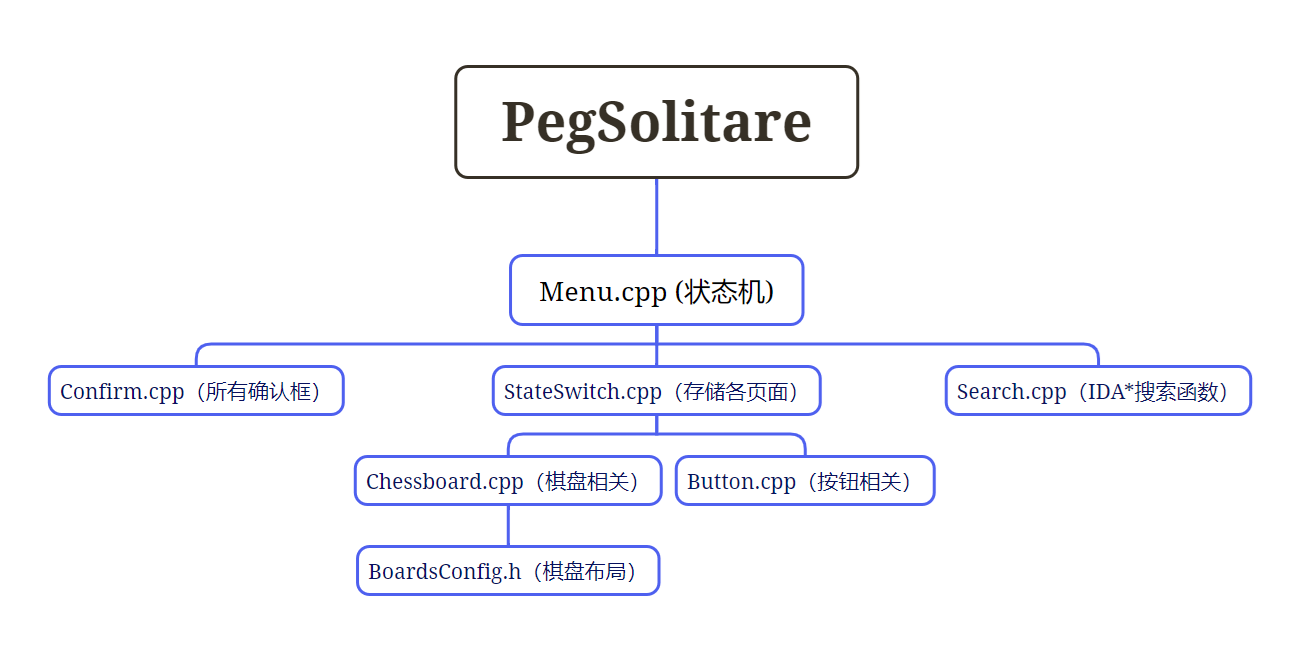
\includegraphics[width=0.7\textwidth]{Orgnazation.png}
  \caption{整体架构}
  \label{fig:architecture}
\end{figure}

\subsection{页面组织关系}
应用入口定义于`Menu.cpp`中的`main`函数,初始化各状态节点的全局对象并启动主循环。页面以状态模式组织:

\begin{itemize}
  \item StateNode基类:定义纯虚方法`render()`和`handleEvent()`。  \item 各具体状态(MainMenuState、ChooseGameState、HowToPlayState、GameState等)继承自StateNode,分别负责菜单、游戏选择、游戏规则、游戏界面等功能。  \item 状态切换由每个节点的`handleEvent()`返回指向下一个StateNode的指针,辅以`StateSwitch.cpp`中的统一调度逻辑。
\end{itemize}
该组织方式使功能模块高度解耦,新增或修改页面只需新增或改写对应的StateNode子类,主框架不受影响。

\begin{lstlisting}
// 状态节点类
class StateNode {
public:
    virtual void render() = 0;
    virtual StateNode* handleEvent() = 0;
    virtual ~StateNode() = default;
};
\end{lstlisting}

\subsection{页面渲染逻辑}
本程序采用面向对象的UI组件设计,所有界面元素如按钮(Button)、标题(Title)、棋盘单元(SingleBlock)等均封装为独立类,负责自身的绘制和状态检测。主循环通过不断获取鼠标位置和点击状态,调用当前状态节点的\texttt{handleEvent()}处理交互事件(如按钮点击、棋子选中、提示生成等),并在事件处理后根据组件内部状态自动更新高亮、选中标识。

当组件的状态或页面内容发生变化时,程序会设置\texttt{needsRender}标志,主循环检测到该标志后先调用\texttt{cleardevice()}清空画面,再调用当前状态节点的\texttt{render()}方法,依次调用各UI组件的\texttt{draw()}或\texttt{drawWithHover()}函数进行重绘,最后通过\texttt{FlushBatchDraw()}一并刷新到屏幕。静态页面(如主菜单、帮助界面、确认弹窗)在鼠标移动时即可触发重绘,以响应悬停效果;游戏主界面仅在鼠标移动幅度超过设定阈值、用户点击或游戏状态变化时才重绘,从而避免无谓的重复绘制,实现性能与体验的平衡。
\begin{lstlisting}
while (current) {

        // 检测鼠标点击事件
        if (currentPressed && !lastPressed) {
            StateNode* next = current->handleEvent();
            if (next != current || current == &gameState) {
                current = next;
                needsRender = true;
            }
        }
        
        // 只在需要时渲染
        if (needsRender && current) {
            current->render();
            FlushBatchDraw();
            needsRender = false;
        }

    }
\end{lstlisting}

\subsection{组件化UI设计}
在UI层面,程序将所有界面元素抽象为组件(Component)实例,每个组件负责自身的渲染和事件响应,典型代表为\texttt{Button}和\texttt{Title}类。此设计借鉴Web前端的CSS样式体系和React的组件化思想:当需要修改按钮或标题样式时,只需在组件内部统一调整,页面中所有实例将即时生效,大大减少了硬编码量并提升了维护效率。
\begin{lstlisting}
    class Button {
private:
    int x, y, width, height;
    const TCHAR* text;
    bool enabled;
public:
    void draw() const; 
    void drawWithHover(int mouseX, int mouseY) const;
    bool isClicked(int mouseX, int mouseY) const;
    bool isHovered(int mouseX, int mouseY) const;
};
\end{lstlisting}
% 之后加一张指出页面中title,button的解释图片,以及加上代码块。
\begin{figure}[h]
  \centering
  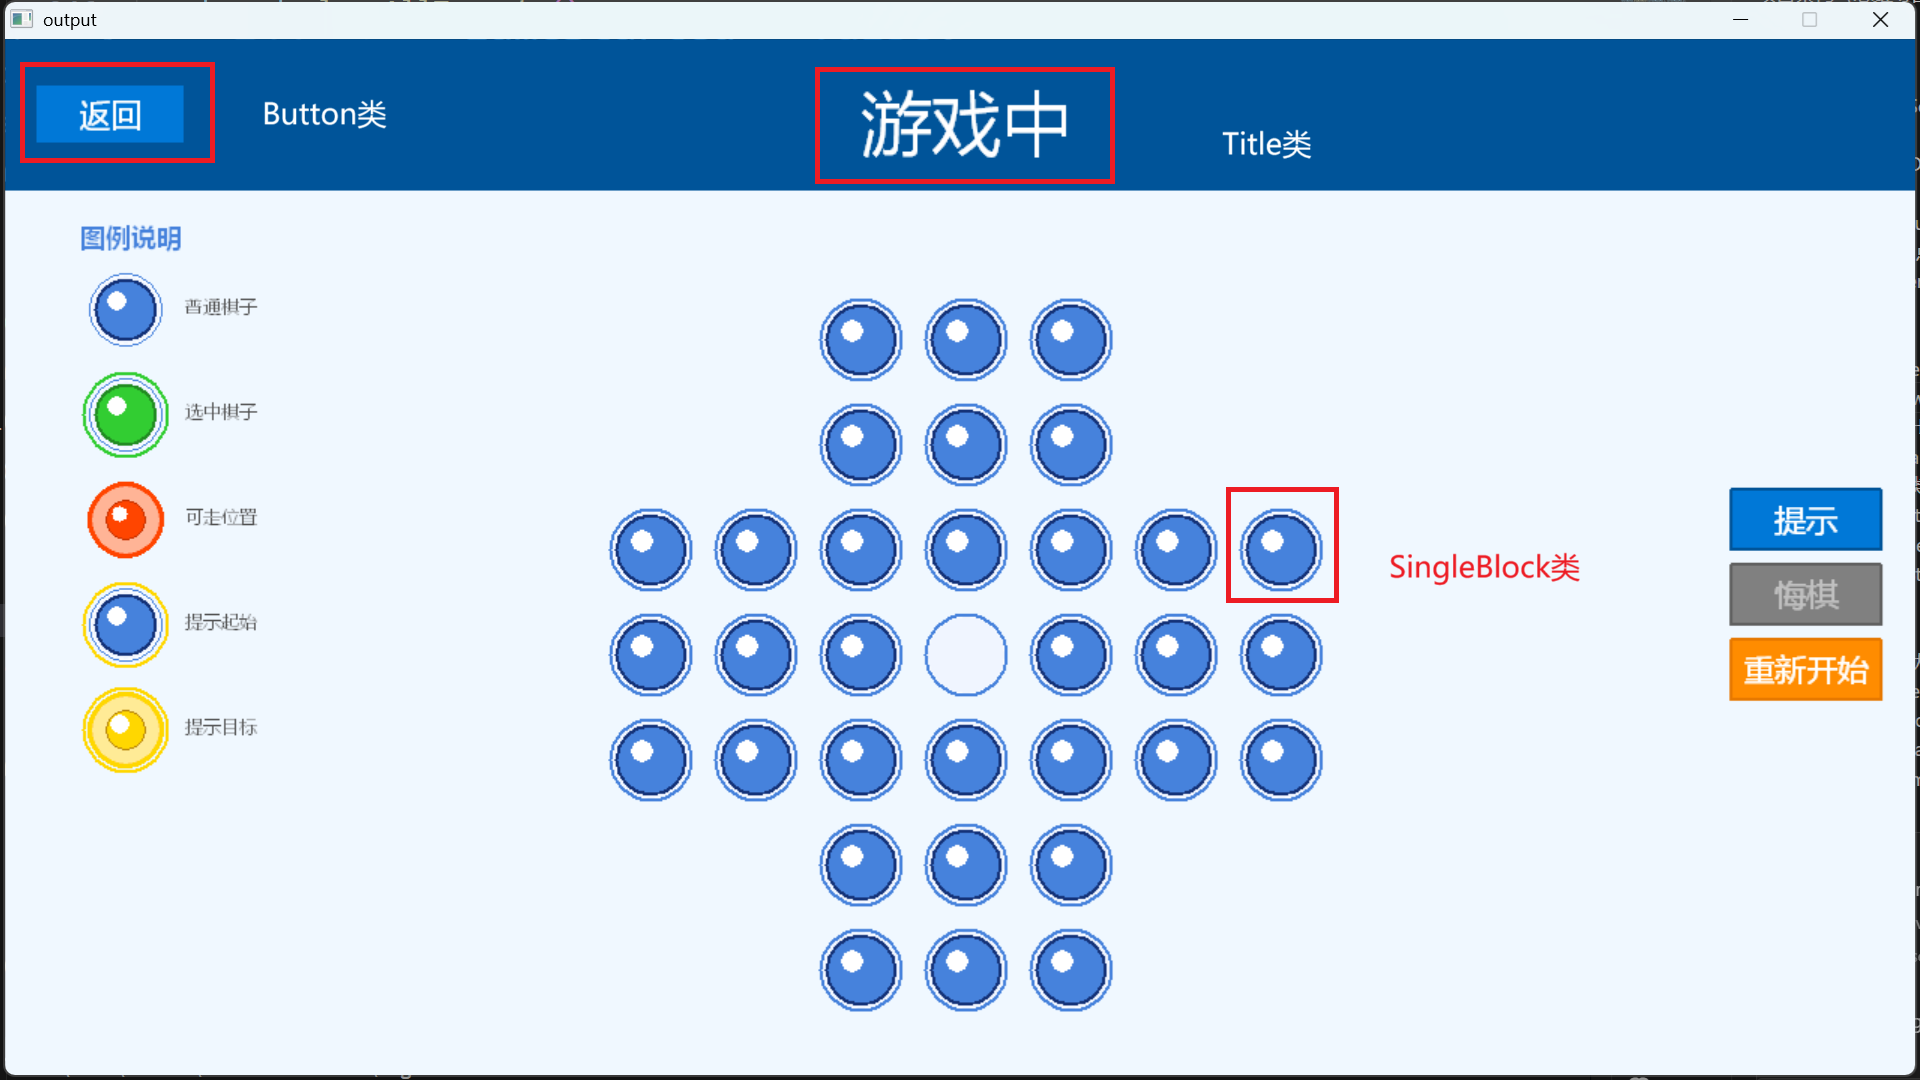
\includegraphics[width=0.6\textwidth]{UIInformation.png}
  \caption{模块化 UI 组件示意图}
  \label{fig:ui-module}
\end{figure}

\subsection{架构优点}
本项目结合状态机模式和函数式编程思想,提升了系统的模块化、可维护性和可测试性。

\textbf{状态机设计的优势:}
状态机将每个界面或逻辑节点封装为独立状态类,render()和handleEvent()职责单一,使页面切换逻辑简洁明了。以GameState为例,用户每次点击棋子即触发选择、移动、提示等状态更新,状态机机制可以灵活响应事件,无需修改主循环。模块化设计便于后期维护,新功能或界面只需添加/修改对应状态类,避免代码侵入。

\textbf{函数式编程风格的优点:}
借鉴React的函数式思想,组件渲染逻辑通过纯函数或无副作用的方法实现,减少了隐藏状态和全局变量的使用。UI组件(如Button、Title、SingleBlock)统一由其自身的render()方法绘制,数据和视图分离,便于组合和复用。同时,纯函数特性使单元测试更加容易,提升了代码可读性和可靠性。


\section{实现细节}
本章将详细介绍程序的核心功能实现,包括UI组件化设计、残局回溯逻辑和搜索算法等,以展示本项目在功能模块划分和逻辑实现方面的思路。

\subsection{组件设计细节}
\texttt{Button}对象内部维护位置、尺寸、文本、颜色和启用状态,调用其\texttt{drawWithHover()}方法结合\texttt{isHovered()}检测鼠标悬停,并动态调整边框颜色和线条粗细,实现高亮效果;\texttt{Title}组件则提供自定义字体和字号选项,并根据窗口宽度自动计算文本居中位置,确保在不同分辨率下标题始终水平居中。

\subsection{页面与弹窗类}
所有页面都封装为独立的类,负责管理自身的UI组件和交互逻辑。\texttt{ConfirmBase}类提供了通用的弹窗框架,通过构造函数的参数灵活配置弹窗的标题、正文、提示文本、背景色、弹窗面板颜色、边框颜色以及确认/取消按钮的样式。
具体弹窗状态如\texttt{ExitState}、\texttt{RestartConfirmState}等继承自\texttt{ConfirmBase},它们在构造函数中只需传入不同的文案和配色,并在\texttt{handleEvent()}方法中实现确认或取消操作的跳转逻辑,即可快速生成完整的对话框界面。该设计将弹窗功能高度抽象化,实现了逻辑复用与样式配置的分离,提高了代码的可维护性和可扩展性。
% 加一张页面的图片

\subsection{渲染刷新逻辑优化}
在主循环中,每次无条件重绘都会造成CPU占用率过高,为此引入以下两项优化策略:

(1) 条件渲染:仅在检测到用户交互(如鼠标点击、键盘输入)或页面内容发生变化时,设置渲染标志并调用\texttt{render()}方法;如若连续迭代期间无任何事件或状态变化,则跳过重绘逻辑。

(2) 帧率限制:在每次循环末尾调用\texttt{Sleep(16)},将刷新频率控制在约60帧每秒,这既能保持界面流畅,又能避免CPU空转浪费。

通过以上优化,程序在保证良好用户体验的同时,显著降低了渲染开销,适用于高性能交互式图形应用。

\subsection{按钮悬停效果实现}
按钮的悬停高亮由 \texttt{Button::isHovered(int mouseX, int mouseY)} 检测鼠标位置,当返回 \texttt{true} 时,\texttt{drawWithHover()} 方法会在原有边框基础上绘制加粗且颜色加亮的光环效果。该逻辑完全封装在组件内部,无需调用方关心细节,保证了界面交互代码的简洁与可维护性。

\subsection{棋盘与棋子的逻辑}
在本项目中,棋盘由一系列\texttt{SingleBlock}对象组成,每个\texttt{SingleBlock}维护坐标(x,y)、尺寸(width,height)以及多个状态标志:
每个格子维护棋子状态、鼠标悬停状态、选中状态以及提示标记等信息,存储于\texttt{Chessboard}的\texttt{std::vector<SingleBlock>}中,并通过相关方法进行状态查询与更新。
\begin{itemize}
  \item \texttt{containsPiece()}/\texttt{setPieceAt(index, bool)}:检查或设置棋子存在;
  \item \texttt{clearAllTargets()}/\texttt{clearAllHintFrom()}:清除所有目标或提示标记;
  \item \texttt{setTargetAt(index, bool)}/\texttt{setHintFromAt(index, bool)}:单个格子目标或提示标记。
\end{itemize}

\subsubsection{棋盘初始化与布局}
棋盘初始化逻辑集中在\texttt{GameState::BoardInit(const std::string\& boardName)}方法中,其主要步骤包括:
棋盘初始化通过预定义的坐标列表加载布局,逐一添加棋盘格子并设置初始棋子状态(通常中心留空),确保棋盘正确渲染并避免重复初始化。
此设计利用集中配置管理多种棋盘类型,仅需在配置文件中添加新坐标,即可支持新布局,无需改动渲染或交互逻辑。

\subsubsection{回溯移动接口}
为支持移动与撤销功能,\texttt{Chessboard}封装了以下核心接口:
\begin{itemize}
    \item \texttt{executeMove(int toIndex)}:根据当前选中块与目标索引计算中间块位置,更新棋盘状态并记录移动历史;
    \item \texttt{undoMove()}:通过弹出移动记录栈顶元素,恢复棋盘至上一步状态;
    \item \texttt{applyReverseMove()}:支持根据当前状态生成并应用合法的反向跳跃集合,用于撤销或分析功能。
\end{itemize}
此结构将布局、移动与回溯逻辑分层封装,便于维护与扩展。

\subsection{残局与回溯功能}
在游戏主界面中,实现了基于移动记录栈的悔棋(Undo)功能。当用户每执行一次合法跳跃,程序内部会创建一条 \texttt{MoveRecord(fromIndex, middleIndex, toIndex)} 记录,并入栈保存移动历史;同时依次调用 \texttt{Chessboard::setPieceAt()} 更新起点、中点和终点的棋子状态。

在渲染阶段,GameState::render 会根据 board.canUndo() 的返回值动态绘制“悔棋”按钮:若为真,则显示高亮可点状态;否则以灰色禁用样式呈现,鼠标悬停不响应。

当用户点击“悔棋”按钮时,GameState::handleEvent 会首先检查 canUndo(),若存在历史记录,则调用 board.undoMove() 弹出上一步操作,并通过 setPieceAt(...) 依次恢复起点和中点的棋子,同时清除终点状态,最后更新界面提示并重绘。
如果回溯至初始状态,\texttt{board.canUndo()} 将返回 false,渲染进入禁用状态,防止继续调用 \texttt{undoMove()} 导致栈空错误。

该设计通过分离状态存储与渲染逻辑,使得回溯功能既安全又易于扩展。\texttt{MoveRecord} 栈可用于实现多步撤销、重做功能或其它历史分析工具。

\subsection{搜索算法的实现}
本项目采用迭代加深A*(IDA*)算法作为搜索核心,结合位运算状态编码和跳跃记录结构,实现孔明棋的智能提示功能。

\subsubsection{IDA* 算法原理与流程}
IDA*算法融合深度优先搜索的空间效率与A*的启发式剪枝优势,主要流程如下:
\begin{enumerate}
  \item 首先计算起始状态 $s_0$ 的启发式估价 $h(s_0)$,通过调用 \texttt{heuristic(start)} 实现,具体为 \texttt{std::bitset<64>(s\_0).count() - 1}。例如英文棋盘初始 32 枚棋子时,$h(s_0)=31$。令 \texttt{bound} = $h(s_0)$,并将 \texttt{nextBound} 初始化为 \texttt{INT\_MAX};
  \item 在当前 \verb|bound| 下调用 \verb|dfs(s, g, bound)|,其中参数 $g$ 表示已执行移动步数,$h$ 为 \verb|heuristic(s)| 返回值。访问每个节点时,计算 $f = g + h$。若 $f > bound$,则执行 \verb|nextBound = std::min(nextBound, f)| 并回溯;否则继续扩展该节点;
  \item 若在遍历中到达目标状态(仅剩一枚棋子),则搜索成功并返回路径;否则遍历结束后,将 \verb|bound| 更新为 \verb|nextBound|,进入下一轮迭代;
  \item 重复上述过程,直至找到解或达到超时/步数限制,保证每轮仅扩展满足 $f \le bound$ 的路径,并逐步逼近最优解深度。
\end{enumerate}

\begin{lstlisting}
    static bool idaStar(State start, std::vector<MoveRecord>& result, int n, const std::vector<Coord>& coords) {
    initMoves(n, coords);
    searchTimedOut = false;
    int bound = heuristic(start);
    while (true) {
        if (searchTimedOut) {
            return false;
        }
        int nextBound = std::numeric_limits<int>::max();
        std::vector<MoveRecord> path;
        if (dfs(start, 0, bound, nextBound, path)) {
            result = path;
            return true;
        }
        if (searchTimedOut) {
            return false;
        }
        if (nextBound == std::numeric_limits<int>::max()) return false;
        bound = nextBound;
    }
}
\end{lstlisting}
\subsubsection{位运算状态编码与移动记录}
为高效表示棋盘状态,程序使用 64 位无符号整数 (\texttt{uint64\_t}) 对棋盘进行编码:
\begin{itemize}
  \item 每个格子对应位图的一位,1 表示有棋子,0 表示空位;
  \item 编码函数 \texttt{encode(st)} 遍历棋盘格子,依据布尔数组构造位图;
  \item \texttt{MoveRecord} 结构体记录一次跳跃的起点、中点和终点索引:
  \begin{verbatim}
struct MoveRecord {
    int fromIndex;    // 起点索引
    int middleIndex;  // 被跳过棋子索引
    int toIndex;      // 终点索引
};
  \end{verbatim}
  \item 程序启动时,调用 \texttt{initMoves(n, coords)} 预生成所有跳跃组合,存入全局容器减少运行时开销。
\end{itemize}

\subsubsection{启发式函数与剪枝策略}
函数 \texttt{heuristic(State s)} 返回当前棋子数减一:
\begin{verbatim}
static int heuristic(State s) {
    return (int)std::bitset<64>(s).count() - 1;
}
\end{verbatim}
该估价满足可承认性和一致性,可在常数时间内估计最少剩余步数。

剪枝策略包括:
\begin{itemize}
  \item 阈值剪枝:当 $f=g+h>bound$ 时,立即回溯并更新 \texttt{nextBound};
  \item 超时控制:记录搜索开始时间,若递归超出预设毫秒数则提前终止;
  \item 重复状态避免:依靠启发式函数减少无效分支,可在路径栈中检测循环。
\end{itemize}

\section{遇到的问题及解决方法}
在开发与测试过程中,项目主要遇到以下问题,并通过相应方式予以解决:
\subsection{页面管理方式的选择}
我认为,在本程序中,最为重要,最为创新的便是该部分。通过状态机彻底改变了底层架构,将本程序与其他程序在本质上区别开来。
起初设计采用独立函数为每个页面渲染和处理事件,不同页面间通过互相调用实现切换。然而在用户反复点击“开始游戏”与“返回”时,函数调用会无限嵌套,最终导致栈溢出和程序崩溃。为解决这一问题,项目改用状态机模式:将每个界面封装为一个状态节点(StateNode),主循环统一调用当前状态的 render() 与 handleEvent() 方法进行渲染与事件响应,再通过状态指针跳转实现页面切换。该设计不仅消除了深度递归的风险,还大幅精简了页面切换逻辑,提高了代码的稳定性和可维护性。

\subsection{游戏画面闪烁}
早期版本中每次循环都进行无条件重绘,导致CPU占用高且界面出现卡顿和闪烁现象。为提升渲染效率与体验,采取了两方面优化措施:

(1) 在主循环中引入 \texttt{needsRender} 标志,仅在检测到鼠标移动、点击或组件状态变化时才执行 \texttt{render()},避免空转重绘。

(2) 启用 EasyX 的双缓冲技术(\texttt{BeginBatchDraw()} 与 \texttt{FlushBatchDraw()}),将所有绘制操作写入后台缓冲区,再一次性刷新到屏幕,彻底消除了闪烁。

上述优化使得游戏主界面在交互和动画场景下均保持平滑流畅,FPS 能稳定在60帧左右,极大提升了用户体验。

\subsection{未定义完时调用自身}
在C++中,若在一个类的声明中就需要使用另一个尚未完全定义的类型(例如持有指向该类型的指针或引用),直接包含其头文件会导致相互嵌套的包含问题。为解决这一“类型未定义完时调用自身”之困,可以使用“前向声明”技术:在使用该类型之前,先在文件开头写上\verb|class OtherType;|,告诉编译器该类型存在但先不展开具体定义。随后在本类中,只需通过指针(\verb|OtherType*|)或引用(\verb|OtherType&|)来使用,即可在编译时通过依赖解析;在实现文件(.cpp)中再包含完整的头文件,获取完整类型信息。这种方法既能解决编译依赖,也有助于降低头文件耦合,缩短编译时间。

\subsection{调试困难及解决方法}
在调试过程中,为明确区分UI渲染与算法执行的异常,我采用了即时状态反馈机制:
\begin{enumerate}
  \item 点击“提示”后,立即调用 \texttt{setStatusText("正在搜索...")} 并刷新界面,确保UI响应正常;
  \item 搜索结束后,根据返回结果更新状态栏为“搜索成功”或“搜索失败”,快速判断算法执行是否出错。
\end{enumerate}
该方案能够迅速定位问题根源,降低调试成本,提升开发效率。

\subsection{状态机架构下的实时渲染}
起初,我的状态机渲染逻辑仅在页面指针发生变化时才触发,这对于菜单、弹窗等静态页面非常有效,但在游戏界面中无法保证实时刷新。为此,我额外引入了对鼠标位置变化的检测:当处于游戏状态且检测到鼠标移动时,即强制触发渲染。这样既避免了无谓的性能开销,又实现了游戏界面的实时渲染。

\section{心得体会}
\subsection{如何高效提示AI}
首先我们必须从根本上了解代码的组织架构,对每一部分的功能有明确的了解。然后我们把大纲列好,再将每一个局部的小函数交给ai实现。提示ai时,最好提示清楚想要的输入输出是什么,以及过程中想用什么样的方法,逻辑来实现。

目前的ai对于这种局部的,目的明确的内容可以写的很好。而对于全局的整体构建,ai則在细节上漏洞百出。相当于是我们给ai提供骨架,ai則在上面填充肉体。因此,目前的ai还离不开我们自己的构思,还是需要对自己的代码有一份清晰的认知,了解每部分的功能,才能最大效率的利用好ai。

\subsection{对类的深刻理解}
原来我只了解了类的大致定义,觉得与结构体相差无几。通过本项目,我学习了多态和继承机制,理解了虚函数的动态绑定原理,并掌握了构造函数、析构函数及拷贝构造函数的用法。这些实践让我深刻体会到面向对象编程的核心思想——封装、继承与多态的结合,使代码更具可扩展性和可维护性,也真正理解了面向对象存在的意义。

\subsection{版本控制与分支管理}
在这次大作业中,我学着使用了 Git 相关的命令进行版本控制。每完成一个小的功能,便执行一次 \texttt{git commit} 进行存档。这样即使之后对原先的代码重构时出现大 Bug,也可以轻松回退到之前的版本,从头开始。
在实现新功能或做重大重构前,会创建分支并进行小步提交和代码审查,保证主干代码的稳定性。

\subsection{模块化设计的重要性}
在正式编码之前,我花时间对整个系统进行模块划分和接口设计。例如,将页面管理、UI 组件、搜索算法和渲染优化等部分分别抽象为独立模块,并定义清晰的交互接口。这样的规划带来以下优势:
模块化设计使我更清晰地掌握项目整体结构,并在开发过程中始终遵循单一职责原则,为后续的维护和升级奠定了坚实基础。
\begin{itemize}
  \item 职责分离:每个模块只负责自身功能,降低了单个文件的复杂度,让项目结构一目了然;
  \item 降低耦合:通过接口调用而非直接依赖,实现模块间松耦合,便于独立开发和测试;
  \item 易于维护与扩展:新增功能时只需在对应模块内修改或新增类,不会影响其他模块;
  \item 提升协作效率:规划好的模块划分有助于多人协同开发,各自专注不同功能,实现并行开发;
  \item 代码复用:通用模块(如按钮、弹窗、棋盘布局等)可在不同页面或项目中复用,减少重复开发。
\end{itemize}

\end{document}